\documentclass[a4paper,12pt]{article}
\usepackage[ngerman]{babel}
\usepackage[utf8]{inputenc}

\usepackage{amsbsy,amsmath,amsthm,amssymb}
\usepackage{amsfonts,enumerate}
\usepackage{verbatim,color}
\usepackage{graphicx}
\usepackage{enumitem}
\usepackage{url}

%\setlength{\oddsidemargin}{-1.cm}
%\setlength{\evensidemargin}{-1.cm}
%\setlength{\textheight}{23.5cm}
%\setlength{\textwidth}{16cm}

\setlength{\topmargin}{-1cm}
\setlength{\textheight}{22.5cm}
\setlength{\textwidth}{16cm}
\setlength{\oddsidemargin}{0cm}
\setlength{\evensidemargin}{0cm}
\setlength{\parindent}{0pt}

\newcommand{\RR}{{\mathbb R}}
\newcommand{\code}{\texttt}

\headsep = 0pt
\textheight = 700pt

\begin{document}
\begin{titlepage}
\centering
\vspace*{5cm}

 \includegraphics[width = 1\textwidth]{LEDtrix_Logo.png}
\vspace{1cm}

\large{Computer Architecture and Operating Systems\\Fall semester 2018}
\end{titlepage}
 
 \section{Introduction}
 
 The LEDtrix is a square LED's matrix inside a box made of wood, connected to RaspberryPi as well as to buttons, to play some games on.
 Our aim is to have at least two games, and code which is expandable so one may easily add a new game.
 The problem will be to efficiently calculate the game-logic, whilst updating the LED's continuously.
 If we do not get this right, the LED's will flicker and therefor worsen the gaming experience.
 Moreover, our buttons are very imprecise, as a result we can not use an interrupt handler on them, but need to demand frequently, whether one has been pushed.
 Besides, depending on where in the gaming process one is, we need to react very differently to the buttons being pressed.
 This may lead to more flickering, consequently we have to look for a good solution.
 
\textbf{Introduction to the topic with a problem statement and questions to examine}
 
 \section{Background}
 
 The idea for our project came by coffee tables containing a LED's Matrix. We liked this and thought of a way to produce something similar, but easier to transport.
 It needed to be robust for which reason we came up with the idea of a wooden box.
 W
 
 \textbf{Introduce and compare relevant technologies, protocols,
algorithms,..}

\section{Building the Box}
We began by building the box, continued by fixating the LED strips and soldering them together.
 Our first problems arouse, when we tried to splice the wooden parts of our box.
 We went to the switch gear workshop of the Elektrizitäts AG Basel to do so, where we realised that this would be very unstable.
 The employees helped us to build the box stronger, by screwing the pieces together, instead of using glue.
 The pictures below show one of the employees helping us to saw the wood (left), and one of us drilling a screw hole into a metal plate, which belongs into one of the corners of the box (right).
 
\vspace{1cm}

{ \centering
  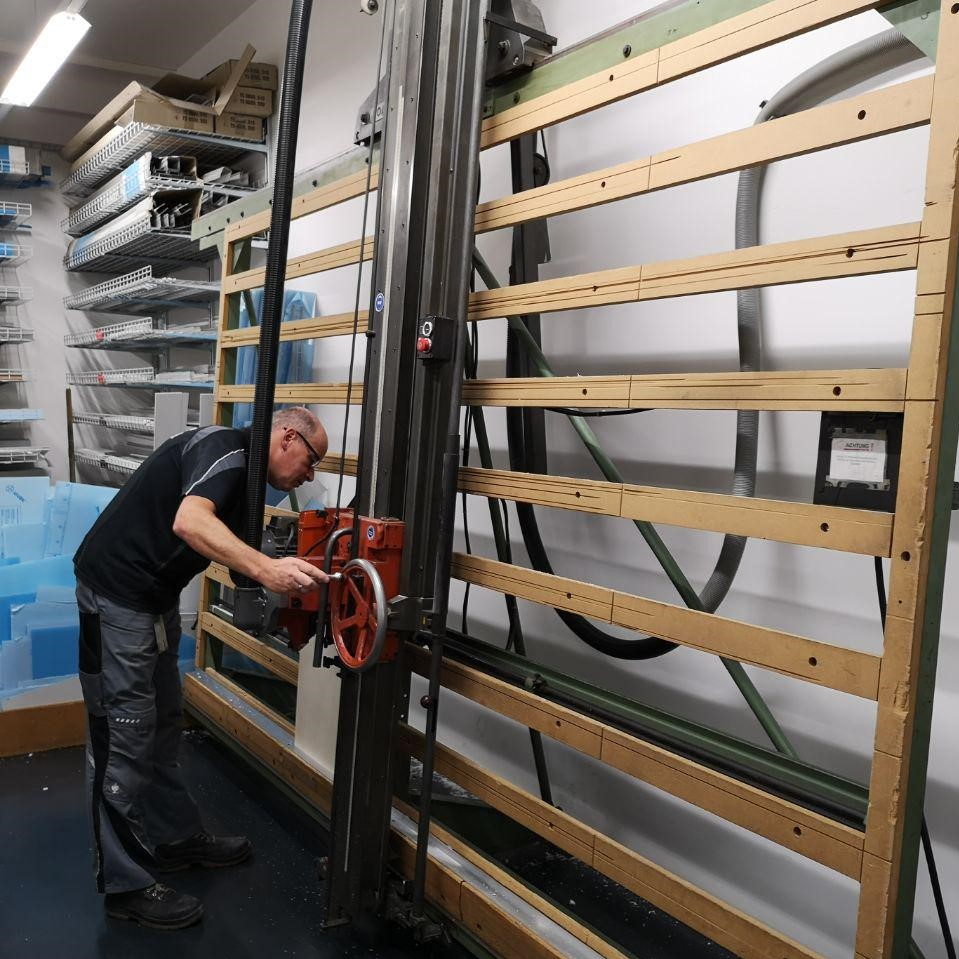
\includegraphics[width = 0.4\textwidth]{brice.jpg}
  \space{   }
  
\includegraphics[width = 0.4\textwidth]{bohren.jpg}
  \\}
 \vspace{1cm}
 
After one day of handicraft work our box was finished, and we ended the day by spraying the outer-wall bright red, what you can see on the picture below (left).
 So the next thing we had to do was to stick the strips onto a wooden board, which you can see us doing so on the picture on the right.
 
 \vspace{1cm}

{ \centering
  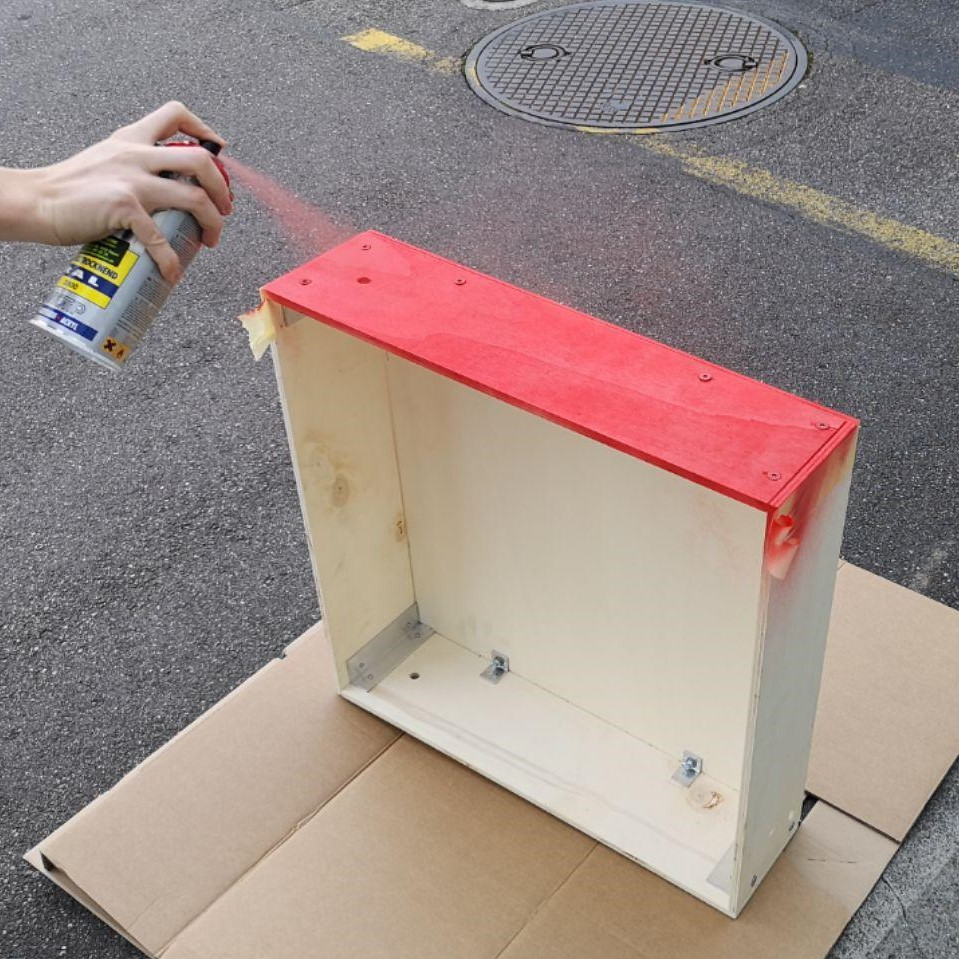
\includegraphics[width = 0.4\textwidth]{sprayen.jpg}
  \space{   }
  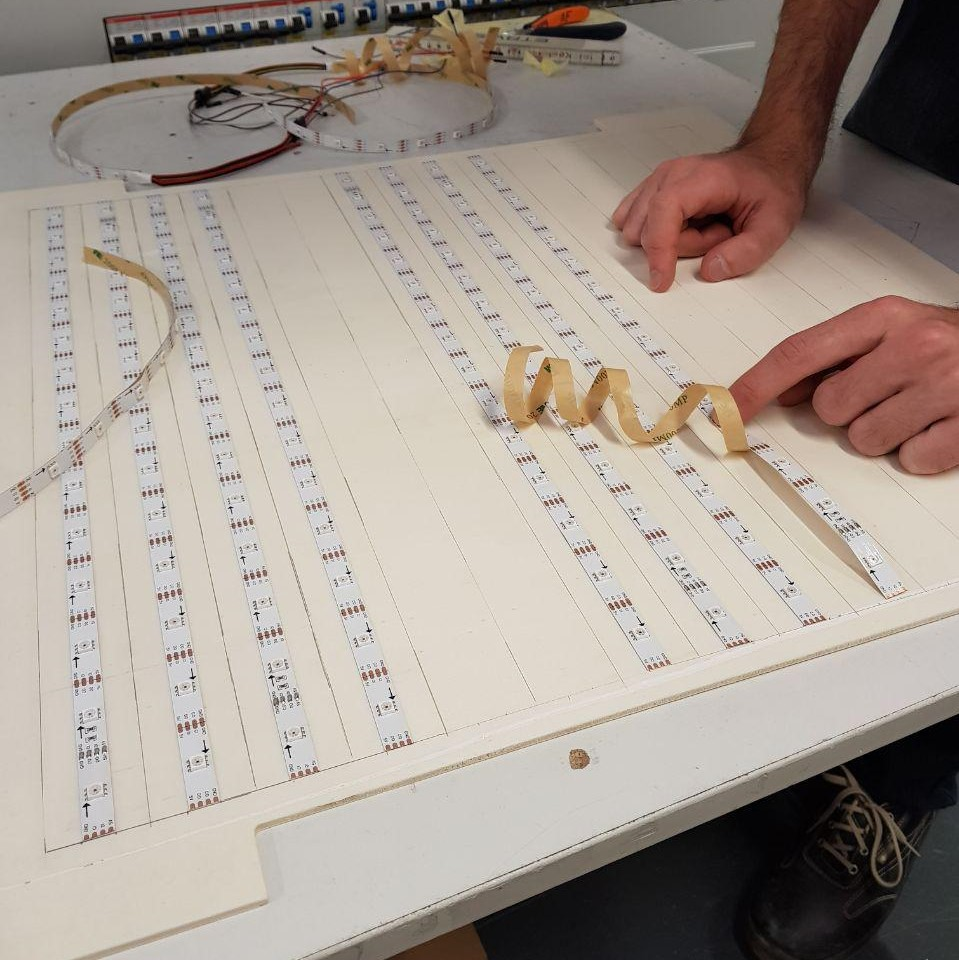
\includegraphics[width = 0.4\textwidth]{kleben.jpg}
  \\}
 \vspace{1cm}
 
After that we had to solder the strips together.
 Since none of us had any experience with soldering, we were surprised how nice it looked and that all of the LED strips were connected and working correctly after the first try.
 Below you see a picture of one of us soldering (left), and the finished LED's board.
 In the beginning we thought about glueing some paper walls between the LED's board and the acrylic glass above it, so we'd have a square for each LED.
 But when we tried it, we both felt it looked nicer without the paper walls, and with no space between the board and the glass, so we did not do that.
 
 \vspace{1cm}

{ \centering
  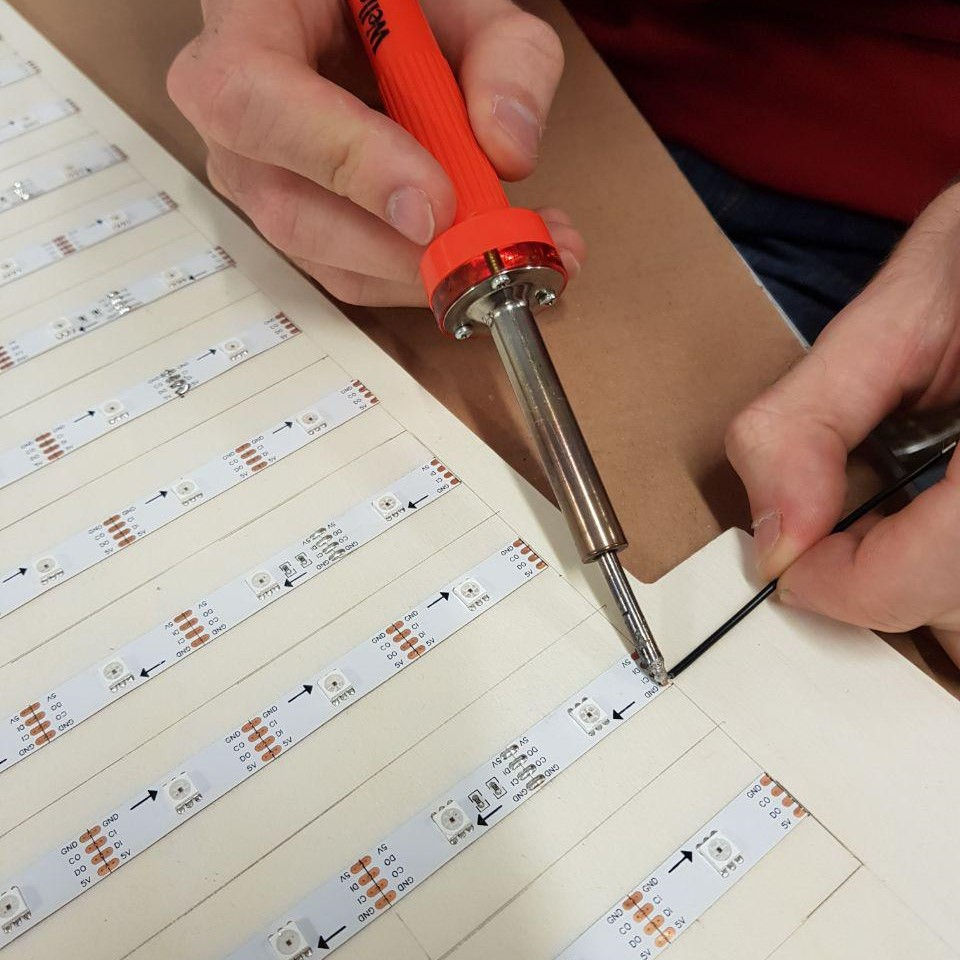
\includegraphics[width = 0.4\textwidth]{loten.jpg}
  \space{   }
  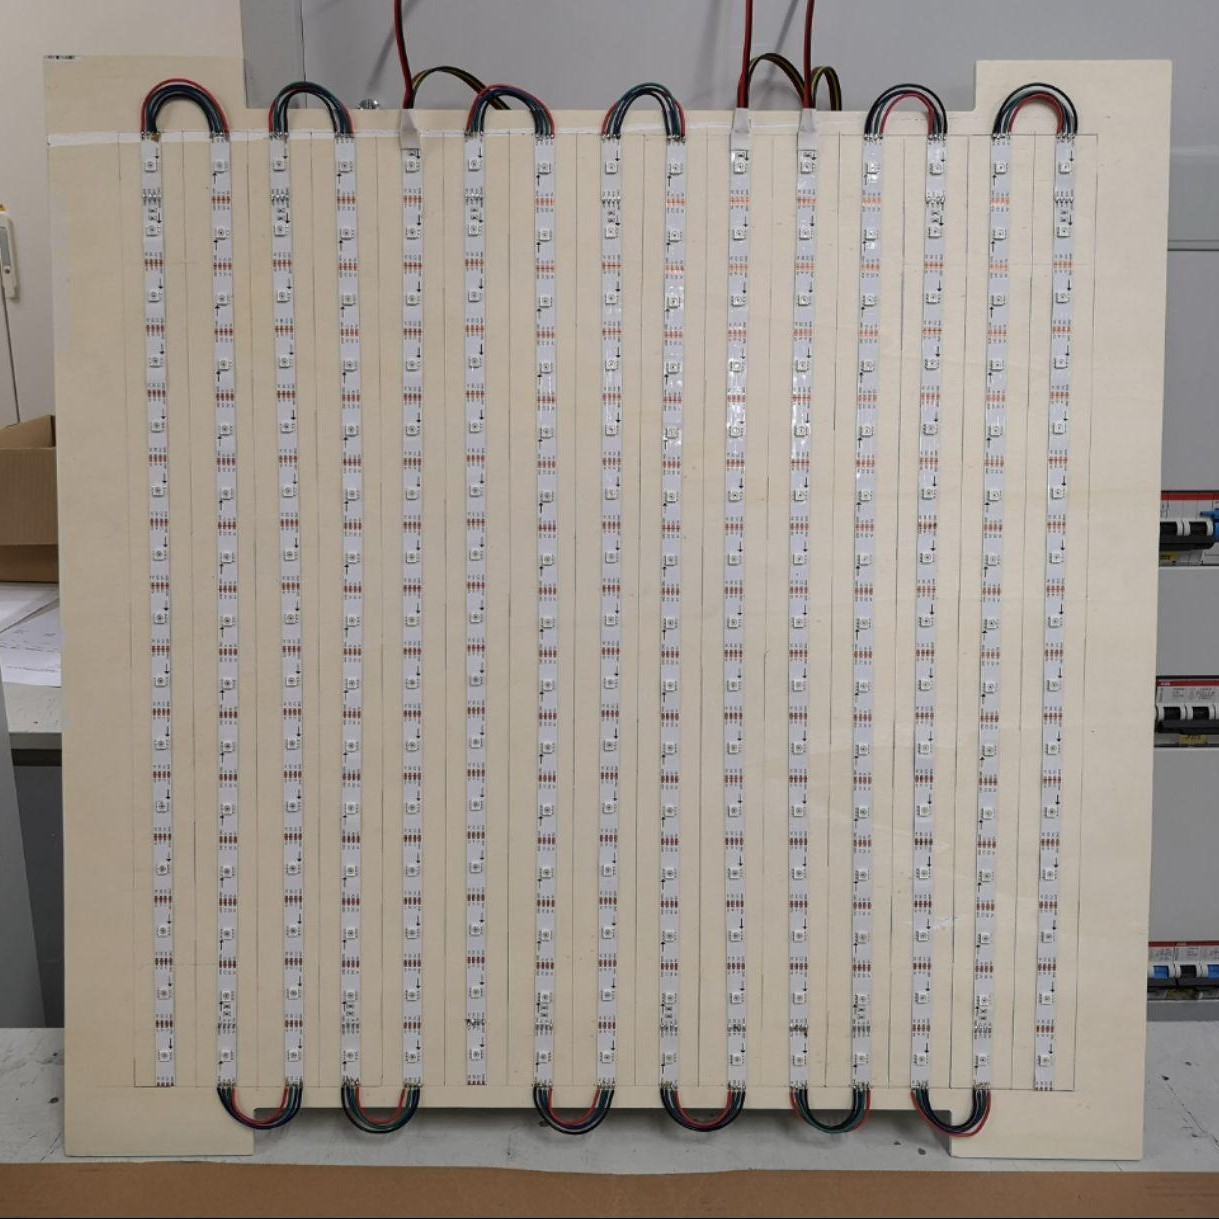
\includegraphics[width = 0.4\textwidth]{matrix.jpg}
  \\}
 \vspace{1cm}
 
\section{Programming}
 We decided on having bools for both buttons, so when a button is pushed, the bool is set to true, and after the information is used, it is set to false.
 This way, we are able to react on the push not by complex switch cases in the button handler, but wherever in the code they are needed.
 
 
Implementation, Configuration and Setup (conceptional, no description
on code-level and no code)

\section{Results}
Graphics, tables, comparisons, insights..

\section{Conclusion}

Discussion/Conclusion/Lessons learned

\section{References}


\end{document}